\documentclass[9pt]{beamer}
\usepackage[utf8]{inputenc}
\usepackage[russian]{babel}
\usepackage{graphicx, epsfig}
\usepackage{subfig}
\usepackage{floatflt}
\usepackage{epic,ecltree}
\usepackage{mathtext}
\usepackage{fancybox}
\usepackage{fancyhdr}
\usepackage{multirow}
\usepackage{enumerate}
\usepackage{epstopdf}
\usepackage{multicol}
\usepackage{algorithm}
\usepackage[noend]{algorithmic}
\def\algorithmicrequire{\textbf{Input:}}
\def\algorithmicensure{\textbf{Output:}}
\usetheme{Singapore}%{Singapore}%{Warsaw}%{Warsaw}%{Darmstadt}
\usecolortheme{default}
\setbeamertemplate{footline}[page number]{}

\usepackage{amsmath,amsfonts,amssymb,amsthm,mathtools} % AMS

\renewcommand{\epsilon}{\ensuremath{\varepsilon}}
\renewcommand{\phi}{\ensuremath{\varphi}}
\renewcommand{\kappa}{\ensuremath{\varkappa}}
\renewcommand{\le}{\ensuremath{\leqslant}}
\renewcommand{\leq}{\ensuremath{\leqslant}}
\renewcommand{\ge}{\ensuremath{\geqslant}}
\renewcommand{\geq}{\ensuremath{\geqslant}}
\renewcommand{\emptyset}{\varnothing}


\newcommand{\ba}{\mathbf{a}}
\newcommand{\bb}{\mathbf{b}}
\newcommand{\bc}{\mathbf{c}}
\newcommand{\be}{\mathbf{e}}
\newcommand{\bp}{\mathbf{p}}
\newcommand{\bq}{\mathbf{q}}
\newcommand{\bt}{\mathbf{t}}
\newcommand{\bu}{\mathbf{u}}
\newcommand{\bw}{\mathbf{w}}
\newcommand{\bx}{\mathbf{x}}
\newcommand{\by}{\mathbf{y}}
\newcommand{\bz}{\mathbf{z}}
\newcommand{\bA}{\mathbf{A}}
\newcommand{\bB}{\mathbf{B}}
\newcommand{\bC}{\mathbf{C}}
\newcommand{\bE}{\mathbf{E}}
\newcommand{\bF}{\mathbf{F}}
\newcommand{\bH}{\mathbf{H}}
\newcommand{\bJ}{\mathbf{J}}
\newcommand{\bP}{\mathbf{P}}
\newcommand{\bQ}{\mathbf{Q}}
\newcommand{\bR}{\mathbf{R}}
\newcommand{\bT}{\mathbf{T}}
\newcommand{\bU}{\mathbf{U}}
\newcommand{\bW}{\mathbf{W}}
\newcommand{\bX}{\mathbf{X}}
\newcommand{\bY}{\mathbf{Y}}

\newcommand{\bbR}{\mathbb{R}}
\newcommand{\bbX}{\mathbb{X}}
\newcommand{\bbY}{\mathbb{Y}}
\newcommand{\bbT}{\mathbb{T}}
\newcommand{\bbU}{\mathbb{U}}
\newcommand{\bbZ}{\mathbb{Z}}

\newcommand{\cA}{\mathcal{A}}
\newcommand{\cD}{\mathcal{D}}
\newcommand{\cL}{\mathcal{L}}

\newcommand{\bepsilon}{\boldsymbol{\varepsilon}}
\newcommand{\bchi}{\boldsymbol{\chi}}
\newcommand{\bnu}{\boldsymbol{\nu}}
\newcommand{\bmu}{\boldsymbol{\mu}}
\newcommand{\btheta}{\boldsymbol{\theta}}
\newcommand{\bTheta}{\boldsymbol{\Theta}}

\newcommand{\T}{^{\text{\tiny\sffamily\upshape\mdseries T}}}

\newcommand{\bOne}{\boldsymbol{1}}
\newcommand{\bZero}{\boldsymbol{0}}
\newcommand{\argmin}{\mathop{\arg \min}\limits}
\newcommand{\argmax}{\mathop{\arg \max}\limits}

\newcommand\undermat[2]{%
	\makebox[0pt][l]{$\smash{\underbrace{\phantom{%
					\begin{matrix}#2\end{matrix}}}_{\text{$#1$}}}$}#2}

\newtheorem{statement}{Утверждение}
\newtheorem{rustheorem}{Теорема}

% отображать название слайда слева
\setbeamertemplate{frametitle}[default][left]

%%% Рисунки
\usepackage{tikz}
\usetikzlibrary{matrix}

%\definecolor{beamer@blendedblue}{RGB}{15,120,80}
%----------------------------------------------------------------------------------------------------------
\title[\hbox to 56mm{  \hfill\insertframenumber\,/\,\inserttotalframenumber}]
{\\ \vspace{1.5cm} Снижение размерности пространства \\ в задачах анализа временных рядов}
\author[Роман Исаченко]{\\ 
	\vspace{.4cm}
	Роман Исаченко \\
	\vspace{3mm}
	{\footnotesize Научный руководитель: \\
	д.ф.-м.н. В. В. Стрижов}}
\institute[МФТИ(ГУ)]{
Московский физико-технический институт\\
Факультет управления и прикладной математики\\
Кафедра <<Интеллектуальные системы>>}
\date{2020 г.}
%--------------------------------------------------------------------------------
\begin{document}
%--------------------------------------------------------------------------------
\begin{frame}
%\thispagestyle{empty}
\titlepage
\end{frame}
%--------------------------------------------------------------------------------
\begin{frame}{Задача декодирования временного ряда}
	\begin{block}{Цель}
		Исследовать зависимости в пространствах объектов и ответов и построить устойчивую модель декодирования временных рядов в случае коррелированного описания данных.
	\end{block}
	\begin{block}{Проблема}
		Целевая переменная -- вектор, компоненты которого являются зависимыми. \\
		Требуется построить модель, адекватно описывающую как пространство объектов так и пространство ответов при наблюдаемой мультикорреляции в обоих пространствах высокой размерности. 
	\end{block}
	\begin{block}{Решение}
		Для учёта зависимостей в пространствах объектов и ответов предлагается снизить размерность с использованием скрытого пространства. 
	\end{block}
\end{frame}
%--------------------------------------------------------------------------------
\begin{frame}{Задача декодирования временного ряда}
	\begin{block}{Цель}
		Исследуется фундаментальная проблема восстановления зависимостей не только в пространстве исходных описаний, но и в пространстве целевых переменных.
	\end{block}
	\begin{block}{Задача}
		Предложить методы поиска скрытых закономерностей в связанных пространствах и алгоритмы снижения размерности, снижения сложности связанных моделей.
	\end{block}
	\begin{block}{Решение}
		Линейные и нейросетевые модели, методы согласования связанных моделей в пространствах высокой размерности.
	\end{block}
\end{frame}
%--------------------------------------------------------------------------------
\begin{frame}{Картинка про работу}
    
\end{frame}
%--------------------------------------------------------------------------------
\begin{frame}{Литература}
	\begin{itemize}
		\item Katrutsa A., Strijov V. Comprehensive study of feature selection methods to solve multicollinearity problem according to evaluation criteria // \textit{Expert Systems with Applications} 76, 2017.
		\vfill
		\item Li J. et al. Feature selection: A data perspective //\textit{ACM Computing Surveys (CSUR)} 50(6), 2017.
		\vfill
		\item Eliseyev A. et al. Iterative N-way partial least squares for a binary self-paced brain–computer interface in freely moving animals //\textit{Journal of neural engineering} 4(8), 2011.
		\vfill
		\item Rodriguez-Lujan I. et al. Quadratic programming feature selection // \textit{Journal of Machine Learning Research} 11(Apr), 2010.
		\vfill
		\item Motrenko A., Strijov V. Multi-way Feature Selection for ECoG-based Brain-Computer Interface // \textit{Expert Systems with Applications} Submitted to the journal.
	\end{itemize}
\end{frame}
%--------------------------------------------------------------------------------
\begin{frame}{Постановка задачи}
	\begin{block}{Модель}
		Назовём \textit{моделью} параметрическую функцию $f: \bbX \times \mathbb{W} \rightarrow \bbY$
	\end{block}
	\begin{itemize}
		\item $\bbX \in \bbR^n$~-- пространство независимой переменной;
		\item $\bbY \in \bbR^r$~-- пространство целевой переменной;
		\item $\bx \in \bbX$~-- реализация независимой переменной;
		\item $\by \in \bbY$~-- реализация целевой переменной;
		\item $\mathbb{W}$~-- пространство параметров модели
	\end{itemize}
	\textbf{Особенностью задачи} является наличие избыточности описания как независимой переменной $\bx$, так и целевой переменной $\by$.
	
	То есть объекты $\bx$ и $\by$ живут на некоторых многообразиях низкой размерности. 
	
	Примером таких многообразий могут являться линейными подпространствами.
\end{frame}
%--------------------------------------------------------------------------------
\begin{frame}{Скрытое пространство}
		
		\begin{itemize} 
			\item
			Назовём пространство $\bbT \subset \bbR^l$ \textit{скрытым пространством} для пространства $\bbX \in \bbR^n$ ($l \leq n$), если существуют \textit{функция кодирования} $\varphi_e: \bbX \to \bbT$ и \textit{функция декодирования} $\varphi_d: \bbT  \to \bbX$ такие что
			\[
			\forall \bx \in \bbX \quad \exists \bt \in \bbT: \varphi_d (\varphi_e(\bx)) = \varphi_d(\bt) = \bx.
			\]
			\item
			Аналогично введём определение \textit{скрытого пространства}~$\bbU \subset \bbR^s$ для целевого пространства $\bbY$, \textit{функции кодирования} $\psi_e: \bbY \to \bbU$ и \textit{декодирования} $\psi_d: \bbU  \to \bbY$
			\[
			\forall \by \in \bbY \quad  \exists \bu \in \bbU: \psi_d (\psi_e(\by)) = \psi_d(\bu) = \by.
			\]
			\item 
			Назовём два скрытых пространства $\bbT$ и $\bbU$ \textit{согласованными}, если существует \textit{функция согласования} $h: \bbT \rightarrow \bbU$, такая что
			\[
				\by = f(\bx) = \psi_d(h(\phi_e(x))).
			 \]
		\end{itemize}
	
\end{frame}
%--------------------------------------------------------------------------------
\begin{frame}{Схема задачи декодирования}
	\begin{figure}
		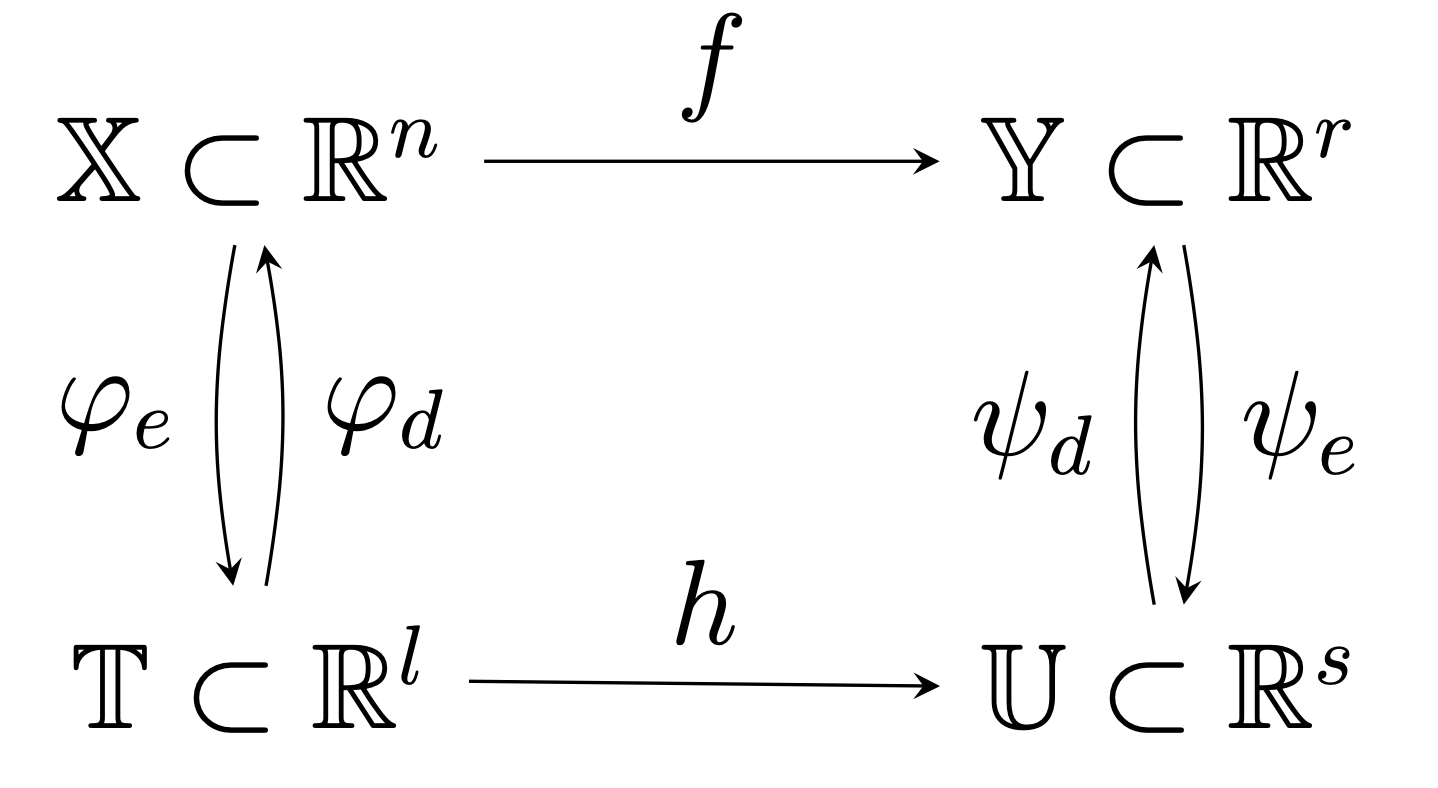
\includegraphics[width=0.5\linewidth]{figs/decoding_scheme}
	\end{figure}
\end{frame}
%--------------------------------------------------------------------------------
\begin{frame}{Многомерная регрессия}
	\begin{block}{Дано}
	$\left( \bX, \bY \right)$~-- выборка, $\bX \in \bbR^{m \times n}$~-- матрица объектов, $\bY \in \bbR^{m \times r}$~-- матрица ответов,
	\[
	\bX = [\bchi_1, \dots, \bchi_n]; \quad \bY =  [\bnu_1, \dots, \bnu_r].
	\]
	\vspace{-0.7cm}
	\end{block}

\begin{block}{Модель}
	\vspace{-0.3cm}
	\[
		\by = \bTheta \bx+ \boldsymbol{\varepsilon}, \quad \bTheta \in \bbR^{r \times n}.
	\]
	\vspace{-0.5cm}
\end{block}
	\begin{block}{Функция потерь}
	\[
	\mathcal{L}(\bTheta | \bX, \bY) = {\left\| \underset{m \times r}{\mathbf{Y}}  - \underset{m \times n}{\bX} \cdot \underset{r \times n}{\bTheta}^{\T} \right\| }_2^2 \rightarrow\min_{\bTheta}.
	\label{eq:error_function}
	\]
	\[
	\bTheta^{\T} = (\bX^{\T} \bX)^{-1} \bX^{\T} \bY.
	\]
	\end{block}
	Линейная зависимость столбцов матрицы~$\bX$ приводит к неустойчивому решению. \\
	Для устранения сильной линейной зависимости предлагается использовать методы выбора признаков и снижения размерности пространства. 
\end{frame}
%--------------------------------------------------------------------------------
\begin{frame}{Снижение размерности пространства}
\begin{block}{Цель}
	\begin{itemize}
		\item спроецировать исходные матрицы $\bX$ и $\bY$ в общее латентное пространство;
		\item максимизировать ковариацию между образами;
		\item сохранить информацию об исходных матрицах.
	\end{itemize}
\end{block}
\begin{block}{Метод частных наименьших квадратов (PLS)}
	\vspace{-0.5cm}
\begin{align*}
\underset{m \times n}{\vphantom{\bQ}\bX} 
&= \underset{m \times l}{\vphantom{\bQ}\bT} \cdot \underset{l \times n}{\vphantom{\bQ}\bP^{\T}} + \underset{m \times n}{\vphantom{\bQ}\bF} 
= \sum_{k=1}^l \underset{m \times 1}{\vphantom{\bp_k^{\T}}\bt_k} \cdot \underset{1 \times n}{\bp_k^{\T}} + \underset{m \times n}{\vphantom{\bp_k^{\T}}\bF},\\
\underset{m \times r}{\vphantom{\bQ}\bY} 
&= \underset{m \times l}{\vphantom{\bQ}\bU} \cdot \underset{l \times r}{\bQ^{\T}} + \underset{m \times r}{\vphantom{\bQ}\bE}
=  \sum_{k=1}^l  \underset{m \times 1}{\vphantom{\bq_k^{\T}}\bu_k} \cdot \underset{1 \times r}{\bq_k^{\T}} +  \underset{m \times r}{\vphantom{\bq_k^{\T}}\bE}.
\end{align*}
\begin{equation*}
\bU \approx \bT \bB, \quad \bB = \text{diag}(\beta_k), \quad \beta_k = \bu_k^{\T}\bt_k / (\bt_k^{\T}\bt_k).
\end{equation*}
\end{block}

\end{frame}
%--------------------------------------------------------------------------------
\begin{frame}{Псевдокод метода частных наименьших квадратов (PLS)}

\begin{figure}
\begin{flushleft}
	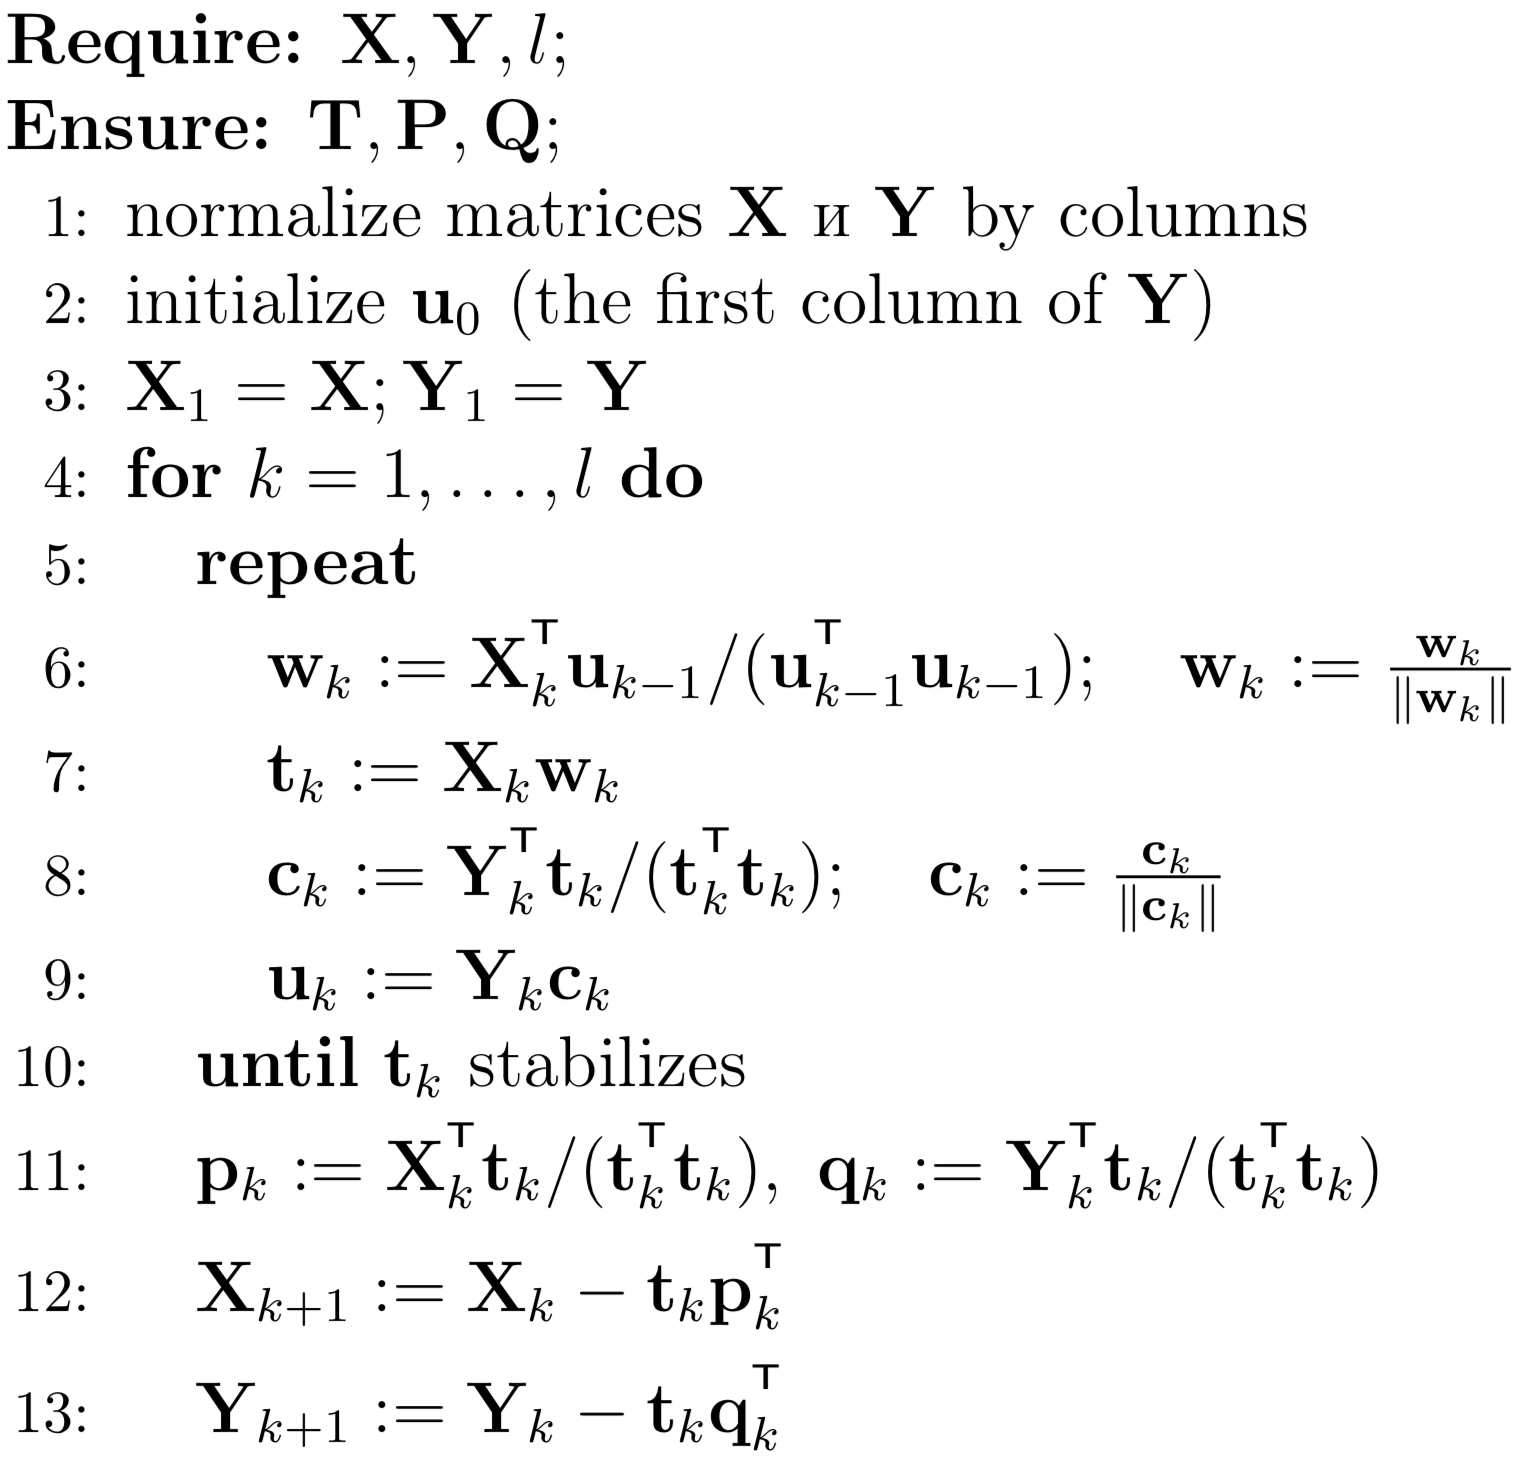
\includegraphics[width=0.6\linewidth]{figs/pls_pseudocode}
\end{flushleft}
\end{figure}
\end{frame}
%--------------------------------------------------------------------------------
\begin{frame}{Метод частных наименьших квадратов (PLS)}

\begin{statement}[Исаченко, 2017]
Максимизация ковариации между векторами~$\bt_k$ и $\bu_k$ приводит к наилучшему описанию матриц $\bX$ и $\bY$ с учётом их взаимосвязи.
\end{statement}
\begin{statement}[Исаченко, 2017]
Вектора $\bw_k$ и $\bc_k$~-- собственные вектора матриц~$\bX_k^{\T} \bY_k \bY_k^{\T} \bX_k$ и $\bY_k^{\T} \bX_k \bX_k^{\T} \bY_k$, соответствуюшие максимальным собственным значениям.
\end{statement}
\begin{statement}[Исаченко, 2017]
Правила обновления векторов (6)--(9) максимизируют ковариацию между векторами~$\bt_k$ и $\bu_k$.
\end{statement}

\begin{block}{Модель PLS регрессии}

\[
\bY = \bU \bQ^{\T} + \bE \approx \bT \bB \bQ^{\T}+ \bE = \bX \bW^* \bB \bQ^{\T} + \bE = \bX \bTheta + \bE.
\]
\vspace{0.1cm}
\[
\bTheta = \bW (\bP^{\T} \bW)^{-1} \bB \bQ^{\T}, \quad \bT = \bX \bW^*, \quad \text{where } \bW^* = \bW (\bP^{\T} \bW)^{-1}.
\]
\end{block}
\end{frame}
%--------------------------------------------------------------------------------
\begin{frame}{Пример PLS регрессии в двумерном случае}
\begin{figure}[h]
\centering
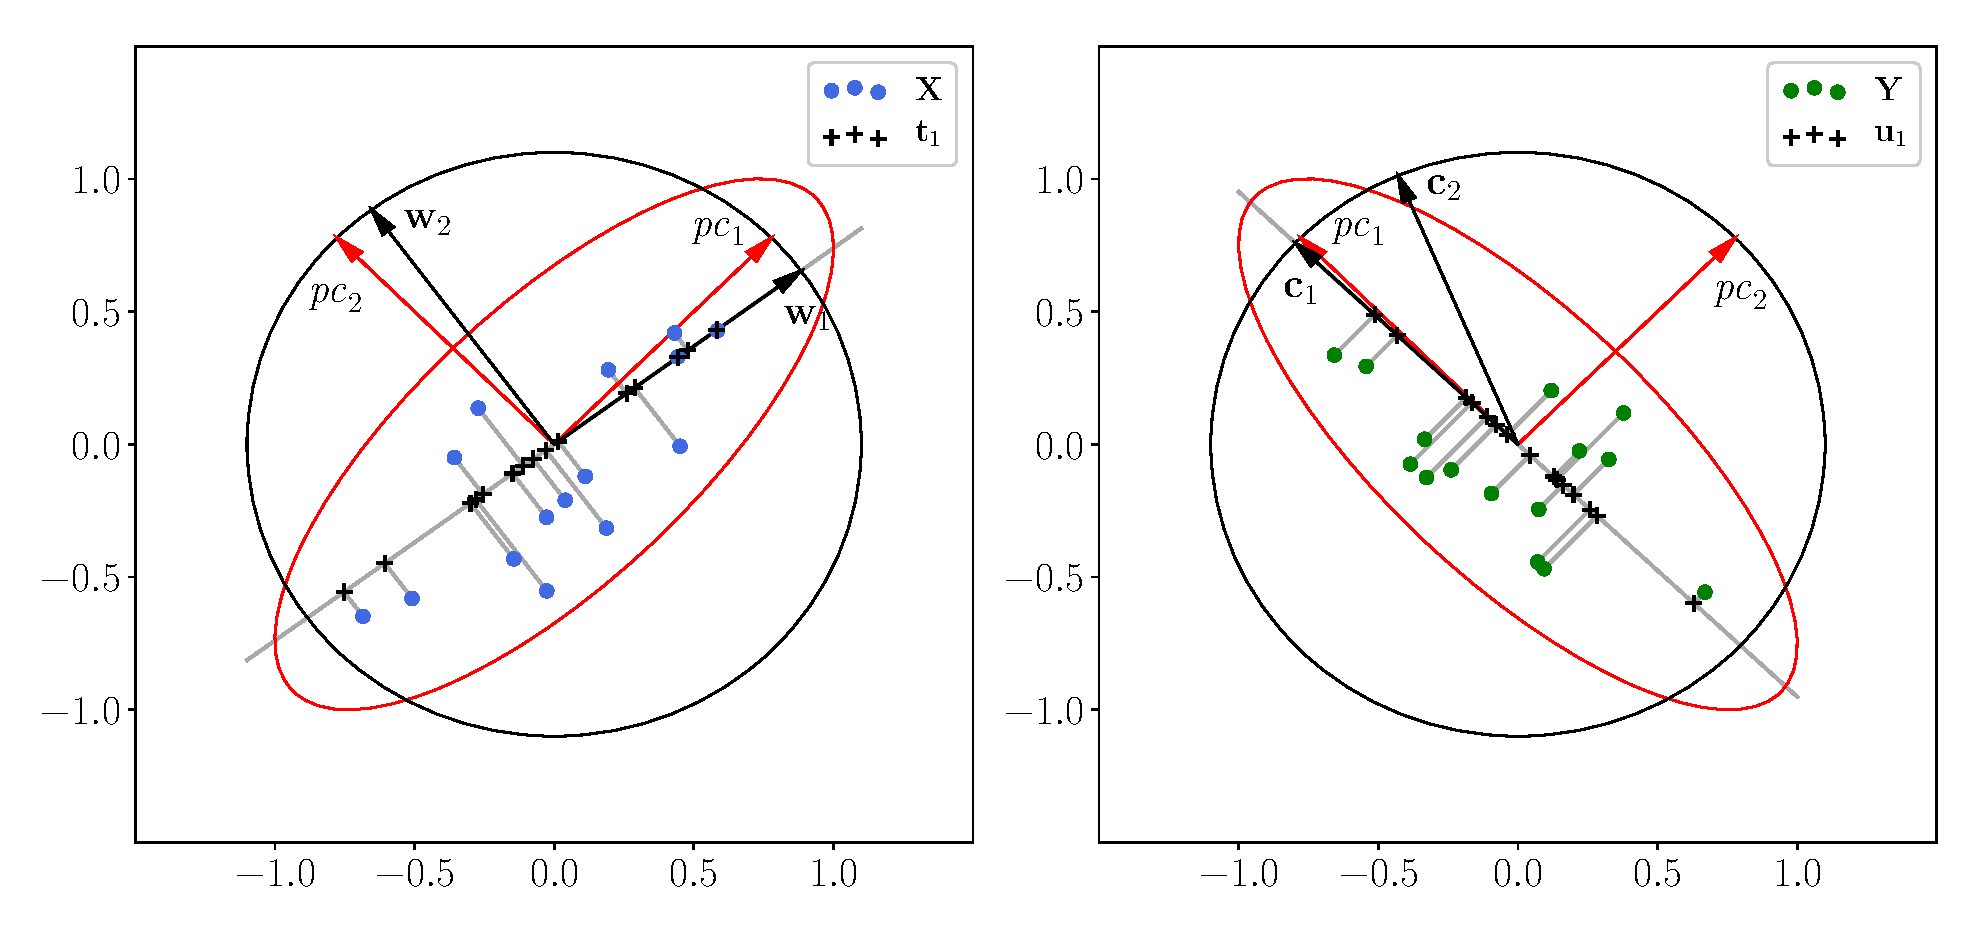
\includegraphics[width=\linewidth]{figs/PLSFigure.eps}
\end{figure}
\end{frame}
%--------------------------------------------------------------------------------
\begin{frame}{Задача выбора признаков}
\begin{block}{Требуется}
Найти бинарный вектор~$\ba = \{0, 1\}^n$, компоненты~-- индикаторы выбранных признаков. 
\end{block}
\begin{block}{Функция ошибки отбора признаков}
	\vspace{-0.2cm}
\[
\ba = \argmin_{\ba' \in \{0, 1\}^n} S(\ba' | \bX, \bY).
\]
\vspace{-0.5cm}
\end{block}
\begin{block}{Релаксация}
	Замена дикретной области определения $\{0, 1\}^n$ на непрерывную релаксацию $[0, 1]^n$:
	\[
	\bz = \argmin_{\bz' \in [0, 1]^n} S(\bz' | \bX, \bY), \quad 
	a_j = [z_j > \tau].
\]
\end{block}
Получив~$\ba$, решаем задачу регрессии:
\[
\mathcal{L}(\bTheta_{\ba} | \bX_{\ba}, \bY) = {\left\| \mathbf{Y} - \bX_{\ba}\bTheta^{\T}_{\ba} \right\| }_2^2 \rightarrow\min_{\bTheta_{\ba}},
\]
где индекс~$\ba$ обозначает подматрицу с номерами столбцов, для которых~$a_j = 1$.
\end{frame}
%--------------------------------------------------------------------------------
\begin{frame}{Quadratic Programming Feature Selection}
	\[
	\| \bnu - \bX \btheta\|_2^2 \rightarrow\min_{\btheta \in \bbR^{n}}.
	\]
	\vspace{-0.3cm}
	\begin{block}{Задача квадратичного программирования}
	\vspace{-0.3cm}
	\[
	S(\bz | \bX, \bnu)	= (1 - \alpha) \cdot \underbrace{\bz^{\T} \bQ \bz}_{\text{Sim}(\bX)} - \alpha \cdot \underbrace{\vphantom{()} \mathbf{b}^{\T} \bz}_{\text{Rel}(\bX, \bnu)} \rightarrow \min_{\substack{\bz \geq \bZero_n \\ \bOne_n^{\T} \bz=1}}.
	\]
	\end{block}
		\begin{itemize}
			\item $\bz \in [0, 1]^n$ -- значимость признаков;
			\item $\bQ \in \bbR^{n \times n}$ -- матрица парных взаимодействий признаков;
			\item $\mathbf{b} \in \bbR^n$ -- вектор релевантностей признаков к целевой переменной.
		\end{itemize}
		\[
		\bQ = \left[\left|\text{corr}(\bchi_i, \bchi_j)\right|\right]_{i,j=1}^n, \quad
		\bb = \left[\left|\text{corr}(\bchi_i, \bnu)\right|\right]_{i=1}^n.
		\]
\vspace{-0.2cm}
\begin{statement}[Исаченко, 2018]
	В случае полуопределенной матрицы~$\bQ$ задача QPFS является выпуклой. 
	Полуопределенная релаксация~-- сдвиг спектра:
\end{statement}
\begin{equation*}
\bQ \rightarrow \bQ - \lambda_{\min} \mathbf{I}.
\end{equation*}
\end{frame}
%--------------------------------------------------------------------------------
\begin{frame}{Многомерный QPFS}
\begin{block}{Агрегирование релевантностей по целевым векторам (RelAgg)}
\[
\bb = \left[\left|\text{corr}(\bchi_i, \bnu)\right|\right]_{i=1}^n \rightarrow \bb = \left[\sum_{k=1}^r\left|\text{corr}(\bchi_i, \bnu_k)\right|\right]_{i=1}^n.
\]
\end{block}
{\bf Недостаток:} нет учёта зависимостей в матрице~$\bY$. 

\begin{block}{Симметричный учёт значимостей (SymImp)}
Штрафуем коррелированные целевые вектора с помощью~$\text{Sim} (\bY)$
\[
\alpha_1 \cdot \underbrace{\bz_x^{\T} \bQ_x \bz_x}_{\text{Sim}(\bX)} - \alpha_2 \cdot \underbrace{\bz_x^{\T} \bB \bz_y}_{\text{Rel}(\bX, \bY)} + \alpha_3 \cdot \underbrace{\bz_y^{\T} \bQ_y \bz_y}_{\text{Sim}(\bY)} \rightarrow \min_{\substack{\bz_x \geq \bZero_n, \, \bOne_n^{\T}\bz_x=1 \\ \bz_y \geq \bZero_r, \, \bOne_r^{\T}\bz_y=1}}.
\]
\[
\bQ_x = \left[ \left| \text{corr}(\bchi_i, \bchi_j) \right| \right]_{i,j=1}^n, \,
\bQ_y = \left[ \left| \text{corr}(\bnu_i, \bnu_j) \right| \right]_{i,j=1}^r, \,
\bB =  \left[ \left| \text{corr}(\bchi_i, \bnu_j) \right| \right]_{\substack{i=1, \dots, n \\ j=1, \dots, r}}.
\]
\[
\alpha_1 + \alpha_2 + \alpha_3 = 1, \quad \alpha_i \geq 0.
\] 
\end{block}
\end{frame}
%--------------------------------------------------------------------------------
\begin{frame}{Многомерный QPFS}
	SymImp штрафует коррелированные целевые вектора, которые в меньшей мере объясняются признаками. 
	\[
	\alpha_1 \cdot \underbrace{\bz_x^{\T} \bQ_x \bz_x}_{\text{Sim}(\bX)} - \alpha_2 \cdot \underbrace{\vphantom{()} \bz_x^{\T}\mathbf{B} \bz_y}_{\text{Rel}(\bX, \bY)} \rightarrow \min_{\substack{\bz_x \geq \bZero_n \\ \bOne_n^{\T}\bz_x=1}}; \quad
	\alpha_3 \cdot \underbrace{\bz_y^{\T} \bQ_y \bz_y}_{\text{Sim}(\bY)} + \alpha_2 \cdot \underbrace{\vphantom{()} \bz_x^{\T} \mathbf{B} \bz_y}_{\text{Rel}(\bX, \bY)} \rightarrow \min_{\substack{\bz_y \geq \bZero_r  \\ \bOne_r^{\T}\bz_y=1}}.
	\]
	\vspace{-0.2cm}
	\begin{block}{Минимаксный подход (MinMax / MaxMin)}
	\vspace{-0.5cm}
	\[
	\min_{\substack{\bz_x \geq \bZero_n \\ \bOne_n^{\T}\bz_x=1}} 	\max_{\substack{\bz_y \geq \bZero_r \\ \bOne_r^{\T}\bz_y=1}} \left(\text {or} \, \max_{\substack{\bz_y \geq \bZero_r \\ \bOne_r^{\T}\bz_y=1}} \min_{\substack{\bz_x \geq \bZero_n \\ \bOne_n^{\T}\bz_x=1}}\right) \left[\alpha_1 \cdot \underbrace{\bz_x^{\T} \bQ_x \bz_x}_{\text{Sim}(\bX)} - \alpha_2 \cdot \underbrace{\bz_x^{\T} \bB \bz_y}_{\text{Rel}(\bX, \bY)} - \alpha_3 \cdot \underbrace{\bz_y^{\T} \bQ_y \bz_y}_{\text{Sim}(\bY)}\right].
	\]
	\end{block}
	\vspace{-0.4cm}
	\begin{rustheorem}[Исаченко, 2018]
		Для положительно определенных матриц $\bQ_x$ и $\bQ_y$ minmax и maxmin задачи достигают одинакового значения функционала.
	\end{rustheorem}
	\vspace{-0.2cm}
	\begin{rustheorem}[Исаченко, 2018]
		Минимаксная задача эквивалентна задаче квадратичного программирования с $n + r + 1$ переменными.
	\end{rustheorem}
	Для получения выпуклой задачи применяется сдвиг спектра.

\end{frame}
%--------------------------------------------------------------------------------
\begin{frame}{Многомерный QPFS}
	\begin{block}{Максимизация релевантностей (MaxRel)}
	\[
		\min_{\substack{\bz_x \geq \bZero_n \\ \bOne_n^{\T}\bz_x=1}} 	\max_{\substack{\bz_y \geq \bZero_r \\ \bOne_r^{\T}\bz_y=1}} \left[ (1 - \alpha) \cdot \bz_x^{\T} \bQ_x \bz_x - \alpha \cdot \bz_x^{\T} \bB \bz_y \right].
	\]
	\end{block}
	\begin{rustheorem}[Исаченко, 2018]
		Для положительно определенной матрицы $\bQ_x$ minmax и maxmin задачи достигают одинакового значения функционала.
	\end{rustheorem}
	\begin{block}{Асимметричный учёт значимостей (AsymImp)}
	\begin{equation*}
	\alpha_1 \cdot \underbrace{\bz_x^{\T} \bQ_x \bz_x}_{\text{Sim}(\bX)} - \alpha_2 \cdot  \underbrace{\left(\bz_x^{\T} \bB \bz_y - \bb^{\T} \bz_y \right) }_{\text{Rel}(\bX, \bY)} + \alpha_3 \cdot \underbrace{\bz_y^{\T} \bQ_y \bz_y}_{\text{Sim}(\bY)} \rightarrow \min_{\substack{\bz_x \geq \bZero_n, \, \bOne_n^{\T}\bz_x=1 \\ \bz_y \geq \bZero_r, \, \bOne_r^{\T}\bz_y=1}}.
	\end{equation*}
	При $b_j = \max\limits_{i=1, \dots n} [\bB]_{i, j}$ коэффициенты при~$\bz_y$ в~$\text{Rel}(\bX, \bY)$ неотрицательны.
	
	\begin{statement}[Исаченко, 2017]
		В одномерном случае $r=1$ предлагаемые стратегии SymImp, MinMax, MaxMin, MaxRel, AsymImp совпадают с исходным алгоритмом QPFS.
	\end{statement}
\end{block}
\end{frame}
%--------------------------------------------------------------------------------
\begin{frame}{Обобщение предложенных методов выбора признаков}
\begin{table}
	\centering
	\footnotesize{
		\begin{tabular}{c|c|c}
			\hline
			Алгоритм & Критерий & Функция ошибки $S(\bz | \bX, \bY)$ \\
			\hline && \\ 
			RelAgg & $\min \bigl[ \text{Sim}(\bX) - \text{Rel}(\bX, \bY) \bigr] $ & $\min\limits_{\bz_x} \bigl[ (1 - \alpha) \cdot \bz_x^{\T} \bQ_x \bz_x - \alpha \cdot \bz_x^{\T} \bB \bOne_r \bigr] $ \\ &&\\
			SymImp & $\begin{aligned} \min \, \bigl[ \text{Sim}(\bX) & - \text{Rel}(\bX, \bY) \\ & + \text{Sim}(\bY) \bigr] \end{aligned}$ & $ \min\limits_{\bz_x, \, \bz_y} \left[ \alpha_1 \cdot \bz_x^{\T} \bQ_x \bz_x - \alpha_2 \cdot \bz_x^{\T} \bB \bz_y + \alpha_3 \cdot \bz_y^{\T} \bQ_y \bz_y \right] $\\ &&\\ 
			MinMax & $\begin{aligned} &\min \, \bigl[ \text{Sim}(\bX) - \text{Rel}(\bX, \bY) \bigr]  \\ & \max \bigl[\text{Rel}(\bX, \bY) + \text{Sim}(\bY) \bigr] \end{aligned}$ & $	\min\limits_{\bz_x} 	\max\limits_{\bz_y} \bigl[\alpha_1 \cdot \bz_x^{\T} \bQ_x \bz_x - \alpha_2 \cdot \bz_x^{\T} \bB \bz_y - \alpha_3 \cdot \bz_y^{\T} \bQ_y \bz_y \bigr]$ \\ &&\\ 
			MaxRel & $\begin{aligned} &\min \, \bigl[ \text{Sim}(\bX) - \text{Rel}(\bX, \bY) \bigr]  \\ & \max \bigl[\text{Rel}(\bX, \bY) \bigr] \end{aligned}$& $\min\limits_{\bz_x} 	\max\limits_{\bz_y} \bigl[ (1 - \alpha) \cdot \bz_x^{\T} \bQ_x \bz_x - \alpha \cdot \bz_x^{\T} \bB \bz_y \bigr]$ \\ 		&&\\
			AsymImp & $\begin{aligned} & \min \, \bigl[ \text{Sim}(\bX) - \text{Rel}(\bX, \bY) \bigr]\\ &  \max \bigl[\text{Rel}(\bX, \bY) + \text{Sim}(\bY) \bigr] \end{aligned}$ & $\min\limits_{\bz_x, \bz_y} \bigl[ \alpha_1 \bz_x^{\T} \bQ_x \bz_x - \alpha_2 \left(\bz_x^{\T} \bB \bz_y - \bb^{\T} \bz_y \right) + \alpha_3  \bz_y^{\T} \bQ_y \bz_y \bigr]$\\  && \\
			\hline
	\end{tabular}}
\end{table}
\end{frame}
%--------------------------------------------------------------------------------
\begin{frame}{Внешние критерии качества}

\begin{block}{Нормированное RMSE}
	Качество предсказания:
	\[
	\text{sRMSE}(\bY, \widehat{\bY}_{\ba}) = \sqrt{\frac{\text{MSE} (\bY, \widehat{\bY}_{\ba})}{\text{MSE} (\bY, \overline{\bY})}} =  \frac{\| \bY - \widehat{\bY}_{\ba} \|_2}{\| \bY - \overline{\bY} \|_2}, \quad \text{где} \quad \widehat{\bY}_{\ba} = \bX_{\ba} \bTheta_{\ba}^{\T}.
	\]
	$\overline{\bY}$~--- константный прогноз.
\end{block}

\begin{block}{Мультикорреляция}
	Среднее значение коэффициента множественной корреляции:
	\[
	R^2 = \frac{1}{r} \text{tr} \left( \bC^{\T} \mathbf{R}^{-1} \bC \right); \quad \bC = [ \text{corr}(\bchi_i, \bnu_j)]_{\substack{i=1, \dots, n \\ j=1, \dots, r}}, \, \mathbf{R} = [ \text{corr}(\bchi_i, \bchi_j)]_{i, j = 1}^n.
	\]
\end{block}
\begin{block}{BIC}
	Компромисс между качеством предсказания и количеством выбранных признаков~$\|\ba\|_0$:
	\[
	\text{BIC} = m \ln \left( \text{MSE} ( \bY, \widehat{\bY}_{\ba})\right) + \| \ba \|_0 \cdot \log m.
	\]
\end{block}
\end{frame}
%--------------------------------------------------------------------------------
\begin{frame}{Вычислительный эксперимент, данные}
\begin{figure}
	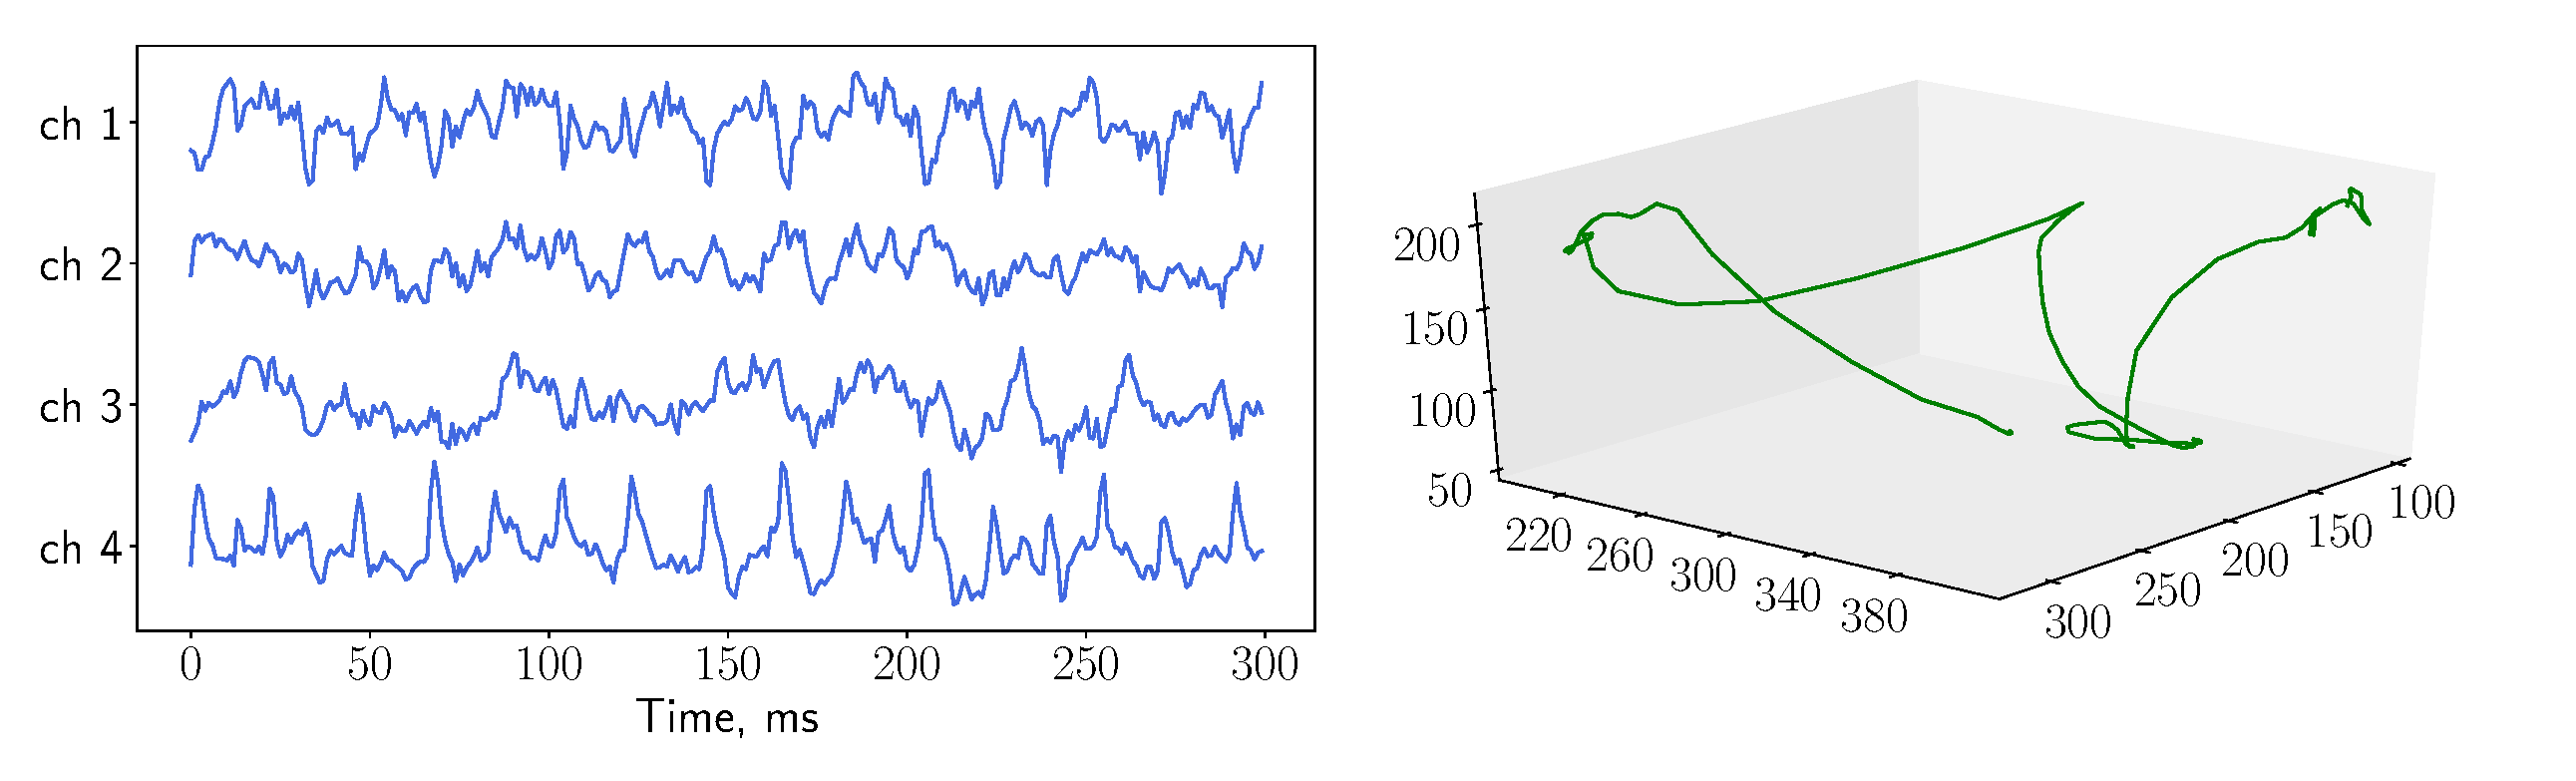
\includegraphics[width=\linewidth]{figs/ecog_data}
\end{figure}
\begin{minipage}{.55\linewidth}
\[
	\bX \in \bbR^{m \times (32 \cdot 27)}; \quad
	\bY \in \bbR^{m \times 3k}.
\]
\vspace{0.1cm}
\[
	\bY = 
	\begin{pmatrix}
	x_1 \,\, y_1 \,\, z_1 & \dots & x_{k\hphantom{+1}} \,\, y_{k\hphantom{+1}} \,\, z_{k\hphantom{+1}}\\
	x_2 \,\, y_2 \,\, z_2 & \dots & x_{k + 1} \,\, y_{k + 1} \,\, z_{k + 1}\\
	 \dots & \dots & \dots  \\
	x_m \, y_m \, z_m & \dots & x_{m + k} \, y_{m + k} \, z_{m + k}
	\end{pmatrix}
\]
\end{minipage}%
\begin{minipage}{.43\linewidth}
	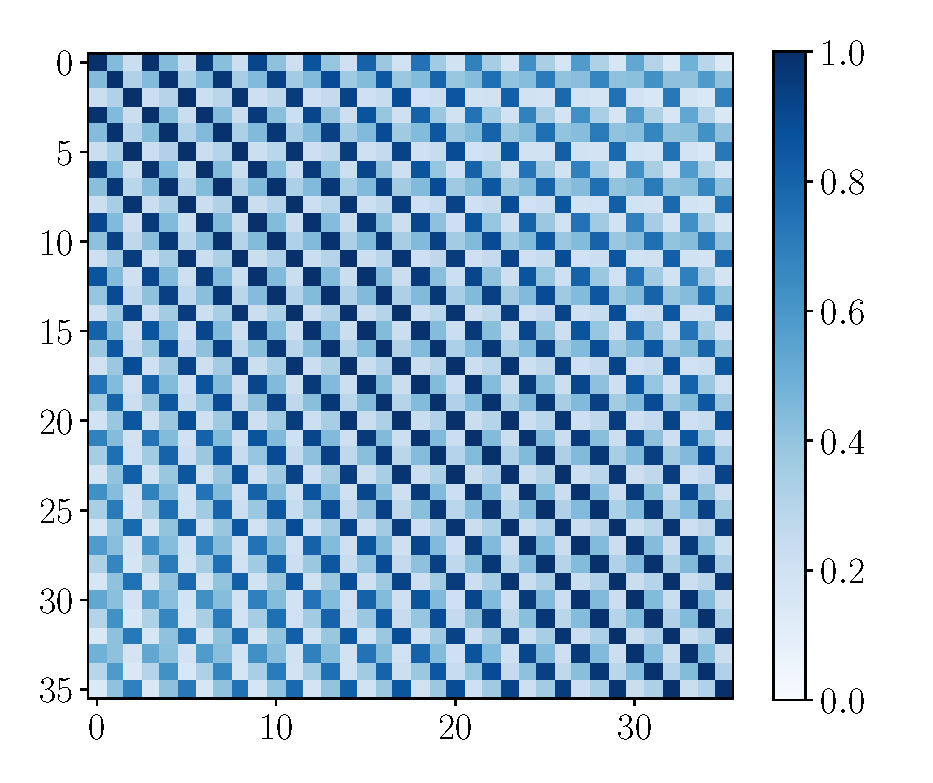
\includegraphics[width=\linewidth]{figs/Y_corr_matrix.eps}
	\begin{center}
		\vspace{-0.4cm}
		Матрица корреляций $\bY$
		\vspace{-0.4cm}
	\end{center}
\end{minipage}
\vspace{0.5cm}

\hrulefill \\
\url{http://neurotycho.org}
\end{frame}
%--------------------------------------------------------------------------------
\begin{frame}{Результаты эксперимента}
	\begin{figure}
		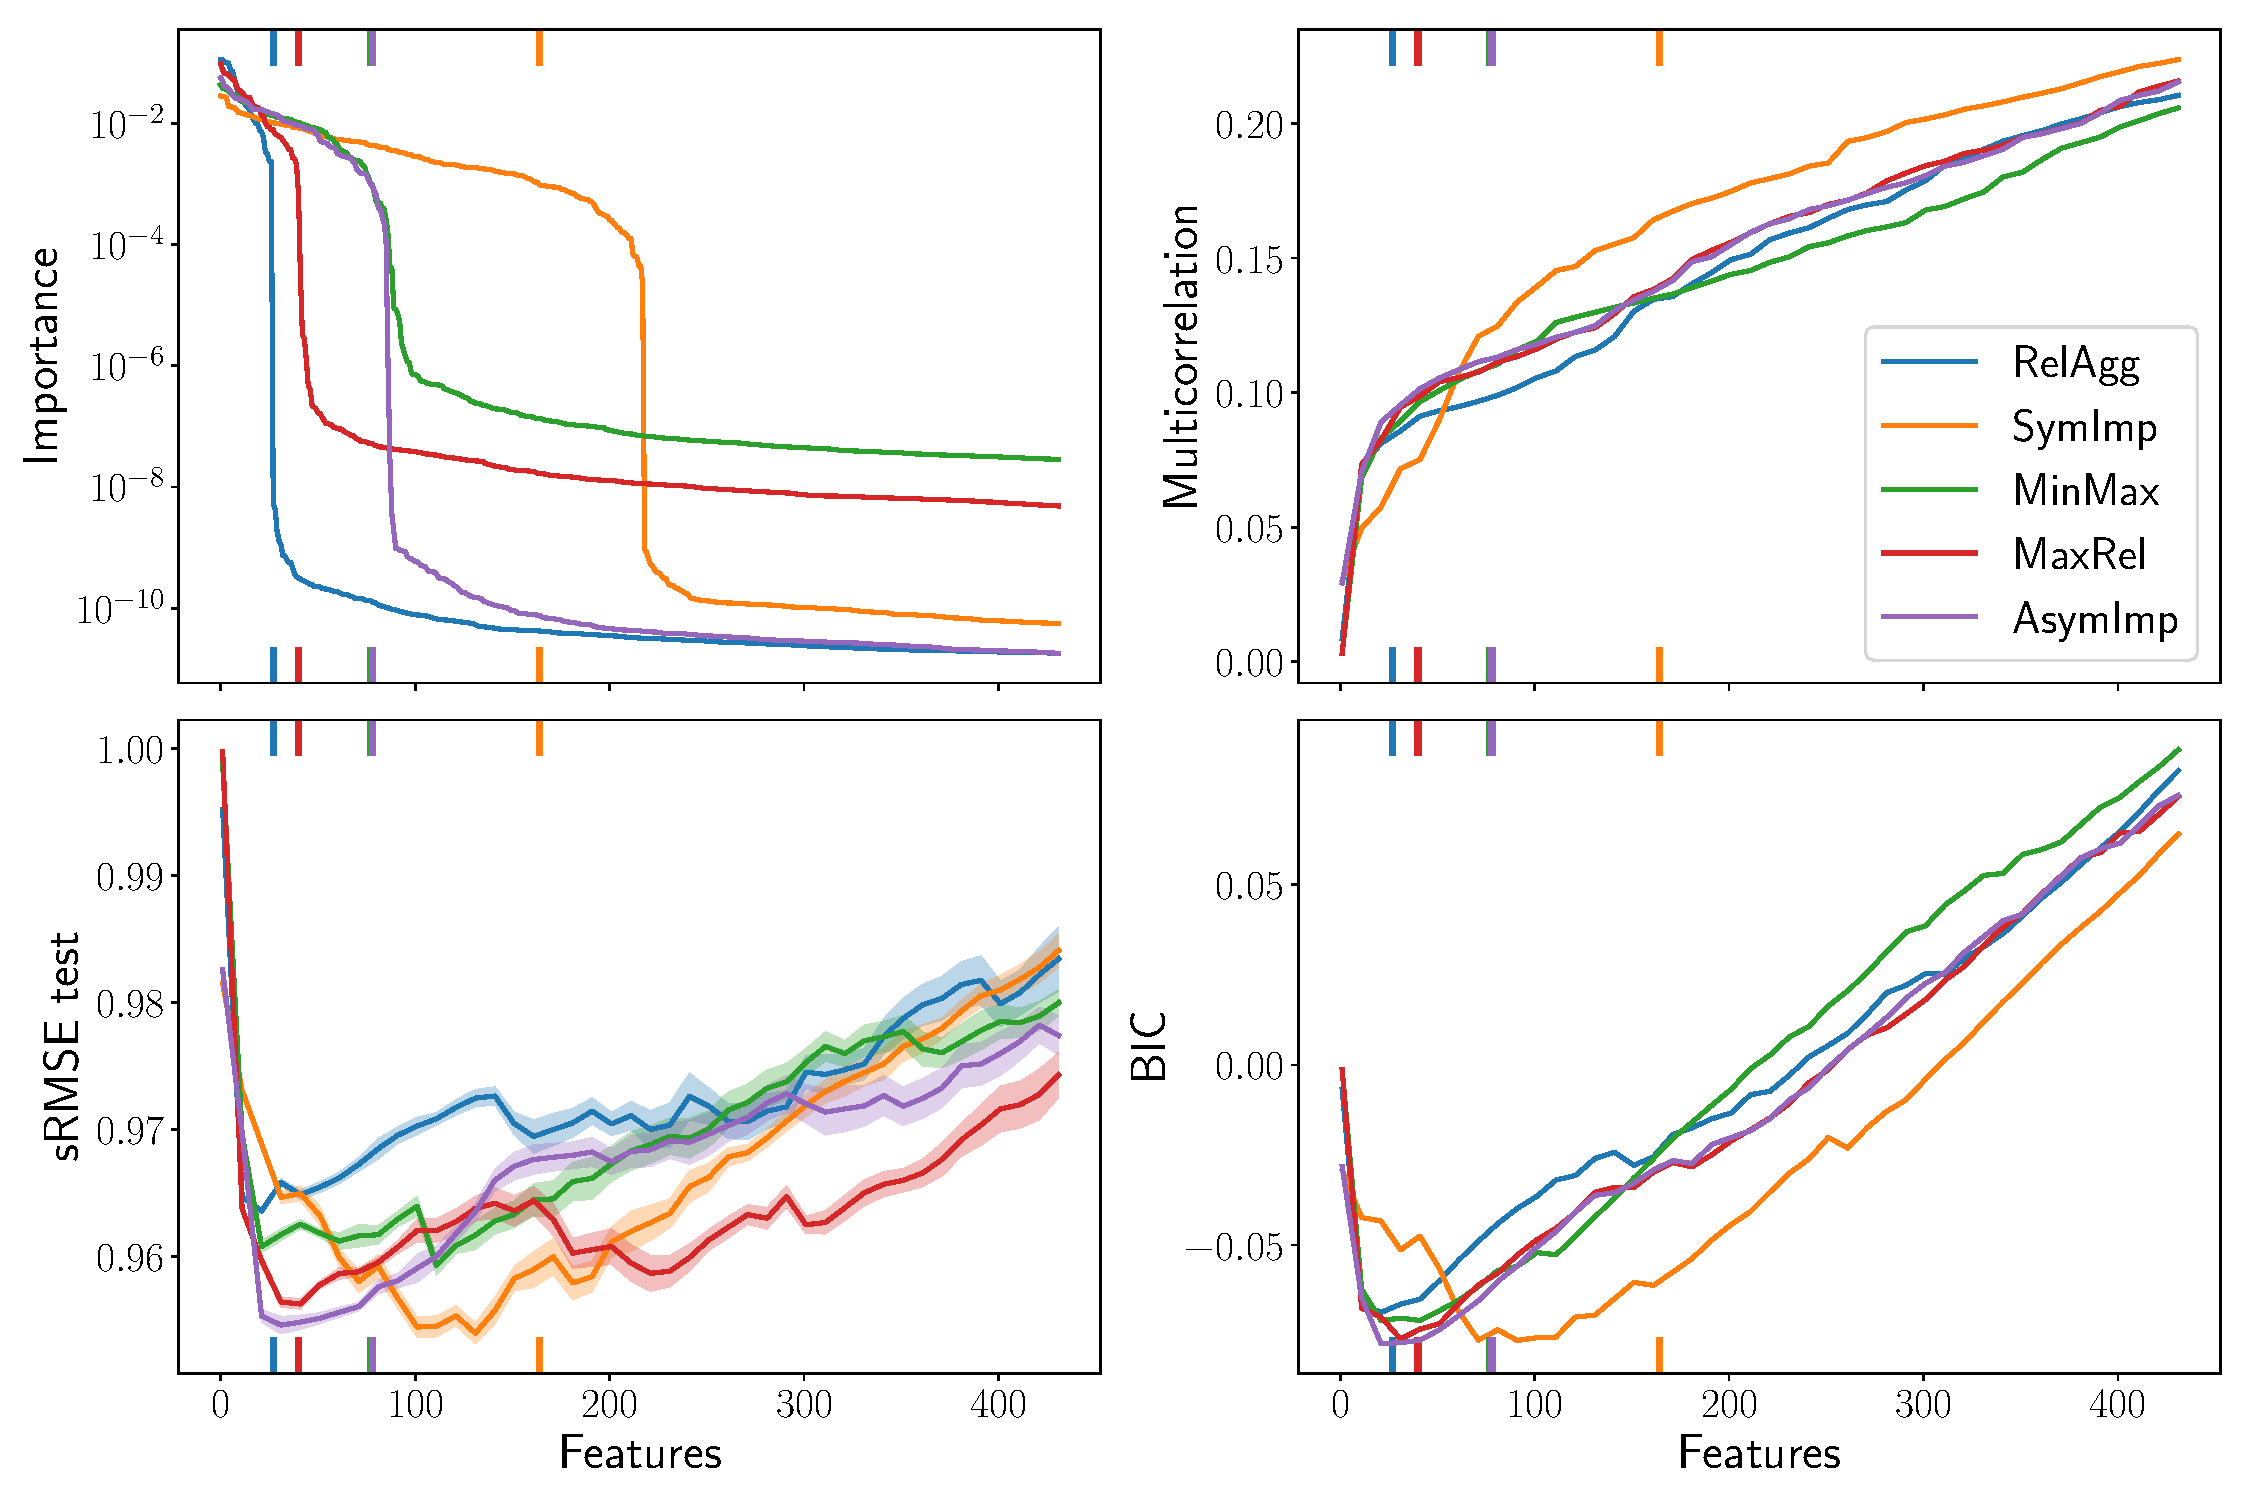
\includegraphics[width=\linewidth]{figs/ecog_3_30_metrics.pdf}
	\end{figure}
\end{frame}

%--------------------------------------------------------------------------------
\begin{frame}{Стабильность выбора признаков}
\begin{block}{Постановка эксперимента}
	\begin{itemize}
	\item cоздать бутстреп-выборки
	\vspace{-0.1cm}
	\[
		(\bX, \bY) \rightarrow \bigl\{(\bX_1, \bY_1), \dots, (\bX_s, \bY_s)\bigr\};
	\]
	\item решить задачу выбора признаков
	\vspace{-0.1cm}
	\[
		 \bigl\{(\bX_1, \bY_1), \dots, (\bX_s, \bY_s)\bigr\}  \rightarrow \{\bz_1, \dots, \bz_s\};
	\]
	\item вычислить статистики
	\vspace{-0.1cm}
	\end{itemize}
	\[
		\{\bz_1, \dots, \bz_s\} \rightarrow \{ \text{sRMSE}, \|\ba\|_0, \text{Спирмен }\rho, \ell_2 \text{ расстояние}\}.
	\]
\end{block}
\renewcommand{\arraystretch}{1.2}
\begin{table}[]
	\centering
	\begin{tabular}{l|ccccc}
		\hline
		& sRMSE  & $\|\ba\|_0$ & Спирмен $\rho$ & $\ell_2$ расстояние \\ \hline
		RelAgg & 0.965 $\pm$ 0.002 & 26.8 $\pm$ 3.8 & 0.915 $\pm$ 0.016 & 0.145 $\pm$ 0.018   \\
		SymImp & 0.961 $\pm$ 0.001 & 224.4 $\pm$ 9.0 & 0.910 $\pm$ 0.017 & 0.025 $\pm$ 0.002   \\
		MinMax & 0.961 $\pm$ 0.002 & 101.0 $\pm$ 2.1& 0.932 $\pm$ 0.009 & 0.059 $\pm$ 0.004   \\
		MaxRel & 0.958 $\pm$ 0.003 & 41.2 $\pm$ 5.2 & 0.862 $\pm$ 0.027 & 0.178 $\pm$ 0.010   \\
		AsymImp & 0.955 $\pm$ 0.001 & 85.8 $\pm$ 10.2& 0.926 $\pm$ 0.011 & 0.078 $\pm$ 0.007  \\ \hline
	\end{tabular}
\end{table}
\end{frame}
%--------------------------------------------------------------------------------
\begin{frame}{QPFS vs PLS}

\begin{block}{Постановка эксперимента}
	 	Сравнить отбор признаков и снижение размерности пространства с помощью моделей линейной регрессии и PLS регрессии.
\end{block}

\begin{figure}[h]
	\begin{minipage}{.43\linewidth}
		\centering
		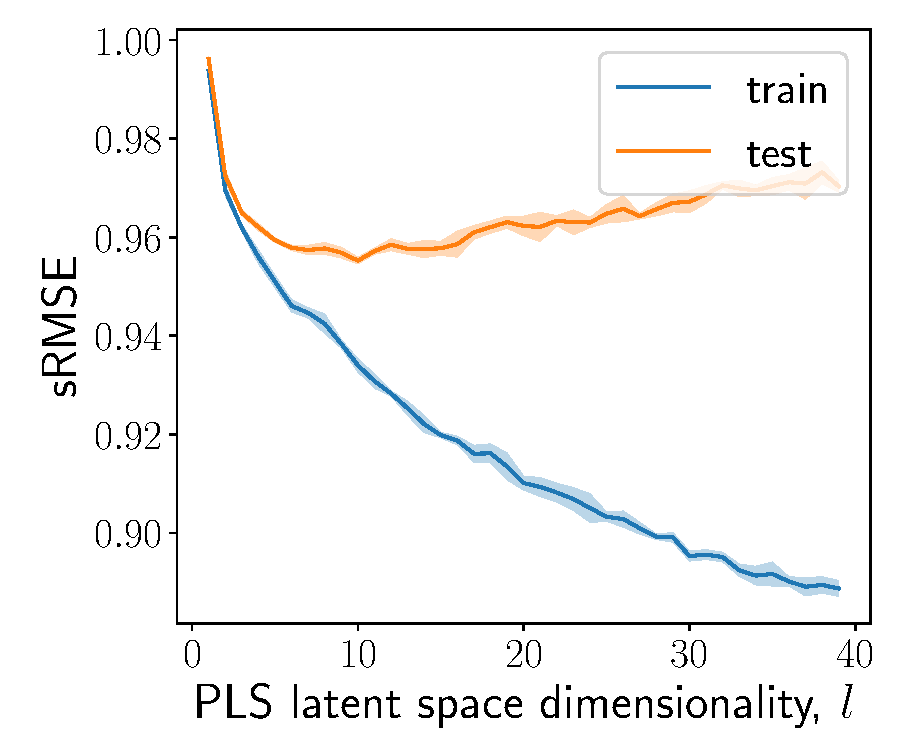
\includegraphics[width=1.\linewidth]{figs/pls_vs_k}
	\end{minipage}%
	\begin{minipage}{.57\linewidth}
		\centering
		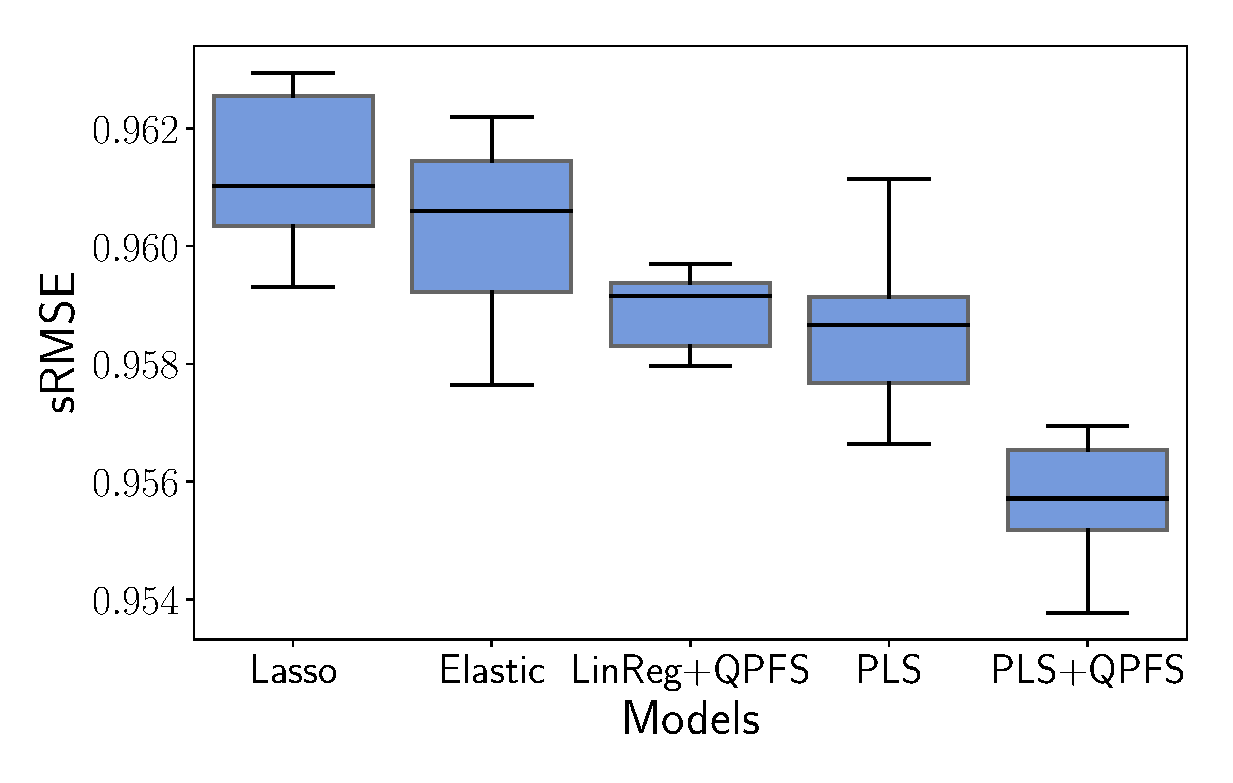
\includegraphics[width=1.\linewidth]{figs/models2}
	\end{minipage}
\end{figure}

\end{frame}
%--------------------------------------------------------------------------------
\begin{frame}{Результаты, выносимые на защиту}
\begin{itemize}
	\item Исследована задача декодирования сигналов в пространствах высокой размерности.
	\vfill
	\item Исследованы методы снижения размерности с анализом структуры пространства.
	\vfill
	\item Предложены методы для выбора признаков, учитывающие зависимости как в пространстве объектов, так и в пространстве ответов.
	\vfill
	\item Предложена комбинация методов выбора признаков и снижения размерности пространства.
	\vfill
	\item Создан макет системы, пригнозирующей сигналы в пространстве большой размерности.
	\vfill
	\item Предложенные алгоритмы выбора признаков доставляют устойчивые и адекватные решения в коррелированных пространствах высокой размерности.
\end{itemize}
\end{frame}
%--------------------------------------------------------------------------------
\begin{frame}{Заключение}
	\begin{block}{Публикации ВАК}
		\vspace{-0.2cm}
		\begin{itemize}
			\item Исаченко Р.В., Стрижов В. В. Метрическое обучение в задачах мультиклассовой классификации временных рядов \emph{Информатика и её применения}, 10(2), 2016.
			\item Isachenko~R. et al. Feature Generation for Physical Activity Classification. \emph{Artificial Intellegence and Decision Making}, 2018, подана в журнал.
			\item Isachenko~R., Strijov~V. Quadratic programming optimization for Newton method. \emph{Lobachevskii Journal of Mathematics}, 2018, принята к публикации.
			\item Isachenko~R., Vladimirova~M., Strijov~V. Dimensionality reduction for multivariate ECoG-based data. \emph{Chemometrics}, 2018, готова к подаче.
		\end{itemize}
	\end{block}
\vspace{-0.2cm}
\begin{block}{Выступления с докладом}
	\vspace{-0.2cm}
	\begin{itemize}
		\item Ломоносов, 2016, Москва. Метрическое обучение в задачах мультиклассовой классификации временных рядов.
		\item Intelligent Data Processing Conference, 2016, Барселона. Multimodel forecasting multiscale time series in internet of things.
		\item Математические методы распознавания образов ММРО, 2017, Таганрог. Локальные модели для классификации объектов сложной структуры.
	\end{itemize}
\end{block}
\end{frame}
\end{document} 
